\documentclass{if-beamer}
\begin{document}
	
	\title[Campus Formoso do Araguaia]{Segurança da Informação}
	\subtitle{Aula 1 }
	\author{Gilmar Gomes do Nascimento}
	\institute[IFTO]{
		Instituto Federal do Tocantins\\
		Campus Formoso do Araguaia
	}
	\date{\today}
	\logo{
		
\includegraphics[scale=0.0085]{logo.jpg}
	}
	\subject{Servers} % metadata
	
	\graphicspath{{figuras/}}
	%---------------------------------------------------------------------------------
	\begin{frame}
		\titlepage
	\end{frame}
	
	\begin{frame}{Catch the flag (Capture a bandeira)}
		\begin{figure}
			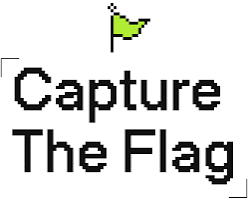
\includegraphics[scale=0.75]{ctf}
		\end{figure}
	\end{frame}
	
	\begin{frame}{Desafios}
		Os desafios em um Capture the Flag geralmente envolvem a descoberta de vulnerabilidades
		 em sistemas operacionais, aplicativos da web, protocolos de rede e outros componentes 
		 de TI. Essas vulnerabilidades podem permitir que atacantes comprometam o sistema, obtenham
		 acesso a informações confidenciais ou executem um código malicioso. 

		 \begin{itemize}
			\item Exploração web
			\item Criptografia
			\item Engenharia Reversa
			\item Forense digital
		 \end{itemize}
	\end{frame}

	\begin{frame}{Lista de CTF}
		Uma lista de \textit{frameworks}, bibliotecas, recursos, programas e tutoriais. Esta lista colabora
		com o aprendizado e compartilhamento de informações sobre CTF.

		\url{https://github.com/apsdehal/awesome-ctf}
	\end{frame}
	
	\begin{frame}{Introdução ao hacking ético e preparação do ambiente}
	Compreender a filosofia do hacking ético diferencia profissionais de cibercriminosos. Além disso, 
	a metodologia Capture The Flag (CTF) torna o aprendizado prático e envolvente. 
	\end{frame}

	\begin{frame}{White Hat}
		Utiliza as mesmas técnicas e ferramentas de um atacante malicioso, mas com a permissão do proprietário
		do sistema e com o objetivo de encontrar e reportar as vulnerabilidades para que possam ser corrigidas.
		É uma atuação proativa que visa fortalecer a segurança antes que os verdadeiros vilões (black hats) apareçam.
	\end{frame}

	\begin{frame}{Mentalidade ofensiva}
		Para defender um sistema, não basta apenas construir muros: é preciso também pensar como quem tentaria derrubá-los.
		 É a partir dessa ideia que a metodologia CTF e o hacking ético ajudam a desenvolver a chamada \textbf{mentalidade ofensiva}.
		\begin{enumerate}
			\item Como isso poderia ser quebrado?
			\item O que acontece se um dado inesperado for enviado?
			\item Existe alguma informação que não deveria estar visível?
		\end{enumerate}
	\end{frame}

	\begin{frame}{OWASP}
		Open Web Application Security Project (OWASP) é uma comunidade on-line global e sem fins lucrativos que produz artigos,  metodologias, documentação, ferramentas e tecnologias de forma livre e aberta no campo da segurança de aplicações web.

	\end{frame}
		 \begin{frame}[allowframebreaks]{Categorias}
			\begin{itemize}
				\item A01: Controle de acesso quebrado (Broken Access Control)
				\item A02: Configuração incorreta de segurança (Security Misconfiguration)
				\item A03: Falhas na cadeia de suprimentos de software (Software Supply Chain Failures)
				\item A04: Falhas criptográficas (Cryptographic Failures)
				\item A05: Injeção (Injection)
			\end{itemize}
		\framebreak
			\begin{itemize}
				\item A06: Design inseguro (Insecure Design)
				\item A07: Falhas de autenticação (Authentication Failures)
				\item A08: Falhas de integridade de software ou dados (Software or Data Integrity Failures)
				\item A09: Falhas de logs de segurança e alerta(Security Logging and Alerting Failures)
				\item A10: Manuseio incorreto de condições excepcionais (Mishandling of Exceptional Conditions)
			\end{itemize}
		\framebreak
		\begin{block}{A01: Controle de acesso quebrado (Broken Access Control)}
		Ocorre quando as restrições sobre o que os usuários autenticados podem fazer não são aplicadas
		de maneira correta, permitindo-lhes acessar dados ou executar ações fora de suas permissões.
		\end{block}
        \begin{block}{A02:Configuração incorreta de segurança (Security Misconfiguration) }
			Resulta da falha em implementar todos os controles de segurança necessários para um servidor ou aplicação web
			 ou da implementação incorreta desses controles.
		\end{block}

		\framebreak

		\begin{block}{A03:Falhas na cadeia de suprimentos de software (Software Supply Chain Failures)}
		 Acontece quando um componente de software, 
		 biblioteca ou dependência de terceiros é comprometido, introduzindo vulnerabilidades na aplicação.
		\end{block}

		\begin{block}{A04:Falhas criptográficas (Cryptographic Failures)}
		 Relaciona-se a falhas na criptografia (ou à sua ausência), que, com 
		 frequência, levam à exposição de dados sensíveis.
		\end{block}
		
		\framebreak

		\begin{block}{A05:Injeção (Injection)}
		Ocorre quando dados não confiáveis são enviados a um interpretador como parte de um comando ou consulta,
		 enganando-o para executar comandos não intencionais ou acessar dados sem autorização.
		\end{block}

		\begin{block}{A06:Design inseguro (Insecure Design)}
		 É uma categoria ampla e representa diversas fraquezas, expressas como ``falta ou ineficácia
		  do controle de design", indicando que os riscos não foram considerados durante a fase de projeto.
		\end{block}
		
		\framebreak

		\begin{block}{A07: Falhas de autenticação (Authentication Failures)}
		acontece quando as funções relacionadas à identidade do usuário, autenticação ou gerenciamento de sessão são implementadas de 
		forma incorreta, permitindo que invasores contornem as proteções.
		\end{block}

		\begin{block}{A08: Falhas de integridade de software ou dados (Software or Data Integrity Failures)}
		 refere-se ao código e à infraestrutura que não protegem contra violações de integridade, como a modificação não autorizada de software ou dados.
		\end{block}
		
		\framebreak

		\begin{block}{A09: Falhas de logs de segurança e alerta(Security Logging and Alerting Failures)}
		significa que a falta de registro, o monitoramento ou o alerta adequados permitem que atividades suspeitas passem despercebidas,
		 dificultando a detecção e a resposta a incidentes.
		\end{block}

		\begin{block}{A10: Manuseio incorreto de condições excepcionais (Mishandling of Exceptional Conditions)}
		 ocorre quando uma aplicação não lida de modo adequado com erros ou outras condições excepcionais, o que pode levar a
		  vazamento de informações ou negação de serviço.
		\end{block}
		
	\end{frame}

\begin{frame}{O papel do Proxy}
	\begin{block}{Definição técnica}
		Atua como um intermediário (``Man-in-the-Middle") entre o navegador e o servidor da aplicação web.
	\end{block}
	\begin{block}{Interceptar}
		O Proxy permite interceptar, visualizar e modificar requisições e respostas HTTPs em tempo real, antes que cheguem ao destino.
	\end{block}
\end{frame}

\begin{frame}{Ferramentas}
	\begin{block}{Na unha}
		O processo de desenvolvimento de código requer técnicas e ferramentas, arcabouços, APIs e 				diversas bibliotecas, técnicas
		de PENTEST idem. É possível criar códigos sem ferramentas? sim, contudo costuma ser bem mais 			complexo e demorado. 
	\end{block}
	\begin{itemize}
		\item OWASP ZAP
		\item BURP
	\end{itemize}
\end{frame}

\begin{frame}{OWASP ZAP}
	\begin{figure}
		
\includegraphics[scale=0.5]{owasp-zap}
	\end{figure}
\end{frame}


	\begin{frame}[allowframebreaks]{Referências Bibliográficas}
		\begin{thebibliography}{9}

		\bibitem{noauthor_undated-xq}
NTP.br. \url{https://ntp.br/conteudo/ntp/}. Acessado em: 6 de agosto de 2026.

\bibitem{Cisco_System_Inc2022-gp}
Cisco System, Inc. (2022). Identificar e Solucionar Problemas do Network Time Protocol (NTP). 26 de setembro de 2022.

\bibitem{ibm}
IBM. (2025). Tivoli Application Dependency Discovery Manager. \url{https://www.ibm.com/docs/pt-br/taddm/7.3.0?topic=problems-synchronization-server}. Acessado em: 6 de agosto de 2026.

\bibitem{cisco}
Cisco. (2025). Use as práticas recomendadas para o Network Time Protocol. \url{https://www.cisco.com/c/pt_br/support/docs/availability/high-availability/19643-ntpm.html}. Acessado em: 6 de agosto de 2026.

\bibitem{suse}
SUSE. (2026). Sincronizando o horário por meio de NTP/NTS. \url{https://documentation.suse.com/pt-br/sle-micro/6.1/html/Micro-ntp-time-synchronization/index.html}. Acessado em: 6 de agosto de 2026.

\bibitem{Moreiras2021}
Moreiras, Antonio Marcos. (2021). NTP e NTS de Forma Correta e Segura, Sincronismo de Tempo na Internet. Nic.br. \url{https://bibliotecadigital.acervo.nic.br/server/api/core/bitstreams/129d1169-25b5-49ce-b015-28ffadc440da/content}. Acessado em: 6 de agosto de 2026.
\end{thebibliography}
	\end{frame}	
	
\end{document}
